\section{Measurements}

\subsection{Baseline Experiment}

In the baseline experiment, we kept Alexa in the office overnight without doing anything and caught up all the package that sent out by Alexa.

In this part, we assume that Alexa will not transfer any voice message to the cloud as there were no voice except some noise generated by nature. Therefore, we could use the package that caught up in this experiment to be the baseline, who were the "necessary" package that Alexa communicate with cloud server. And we assume them to be unsuspicious package, which include some handshake package and broadcast package to let the Alexa confirm which server to communicate with.






\subsection{"Prefix" Experiment}

As Amazon has mentioned in his document \todo{[1]}: "By default, Alexa-enabled devices only stream audio to the cloud if the wake word is detected (or Alexa is activated by pressing a button)." it will not transmit any data before the wake up word. In order to test out this announcement, we let Alexa to start transmitting the voice to the server. 

Therefore, in this part, we did two different kinds of experiments. First, we played a voice contained with a prefix sentence as well as a command and another voice without prefix sentence but just command for Alexa. The prefix sentence is a random sentence that simulates a person talking in his daily life, and then he asked Alexa a question. It is really common in our daily life that people just having some conversation and suddenly find something to deal with, therefore they send a command to Alexa. The whole prefix sentence is: " I think I am having some trouble hearing what people trying to say to me. I am not feeling particularly well now. I am also thinking switching a new job." and it played for 9 seconds. The command is: "Alexa, where is New York City." and it played for 2.5 seconds. As a result, if Alexa did record some part of the prefix sentence, the package size of these two parts would show up a significant difference.

Further, we played a voice with the prefix sentence and ranged the time from 9s to 0s, then followed by a 2.5 seconds command to wake Alexa up and let it transmit the package and answer. Our assumption is that, if Alexa truly did the transmission as it mention, the size of each transmission package should be the same, as there is only a short command at the end of the sentence. However, if the optimization algorithm of Alexa is not efficient enough, it might transmit some parts of the prefix sentence to the cloud and the package size would wave all the night.
 

\begin{figure}[]
    \centering
    \includegraphics[width=\linewidth]{1204/outgoing_data_size_vs_prefix_time.png}
    \caption{Plot of the total outgoing data size against the length of non-command speech played immediately before a command. The error bars extend to one standard deviation in either direction. Total outgoing data size is calculated as the sum of the TLS packet payload lengths going to the destination IP address with the greatest such sum.}
    \label{fig:prefix_many}
\end{figure}

\begin{figure}[]
    \centering
    \includegraphics[width=\linewidth]{1205/outgoing_data_size_vs_prefix_time.png}
    \caption{\todo{Should probbaly be a bar graph, if present at all. Alternately, side-by-side histograms may be effective}. Plot of the total outgoing data size against the length of non-command speech played immediately before a command. The error bars extend to one standard deviation in either direction. Total outgoing data size is calculated as the sum of the TLS packet payload lengths going to the destination IP address with the greatest such sum.}
    \label{fig:prefix_two}
\end{figure}








\subsection{"Postfix" Experiment}
  
Moreover, we want to measure whether Alexa will keep transmitting package even if Alexa has noticed the whole command and started replying. The assumption here is that, as Alexa has started replying, it means Alexa has fully recognized the whole command and it should not transmit the rest of the sentence onto the server. The experiment fits our real life situation that someone sends a command to Alexa and starts another conversation with others immediately. If Alexa transmits the rest of the conversation, it would definitely rises the privacy concern.

Here, we use "Alexa, where is New York City" as a command sentence and adds a 1 second postfix sentence. We gave an approximately 0.5 seconds gap between the command and postfix sentence to simulate the normal silent gap when people finished a sentence. Then we started playing three different kinds of sentences which are: a) command voice b) command voice with 0.5 second postfix sentence and c) command voice with 1 second postfix sentence. And analyze the package sent out by Alexa.

\begin{figure}[]
    \centering
    \includegraphics[width=\linewidth]{1206/extra_filtered_outgoing_data_size_vs_prefix_time.png}
    \caption{\todo{Should probbaly be a bar graph, or maybe histograms, but I think three histograms is too many}. Plot of the total outgoing data size against the length of non-command speech played 0.5 s after a command. The error bars extend to one standard deviation in either direction. Total outgoing data size is calculated as the sum of the TLS packet payload lengths going to the destination IP address with the greatest such sum.}
    \label{fig:postfix_gap}
\end{figure}



What's more, we want to see whether that 0.5 second silence gap between command and postfix sentence is necessary for Alexa to realize the command is over. Here, we played the command with postfix sentence immediately (i.e. delete the silence gap between postfix sentence and command.). We try to find out whether Alexa would automatically cut off the voice once it recognized the following sentence is meaningless. We played command with 0,1,2,3 seconds postfix sentence, which contains nonsense sentences, to see whether Alexa would cut off the transmission itself.


\begin{figure}[]
    \centering
    \includegraphics[width=\linewidth]{1207/extra_filtered_outgoing_data_size_vs_prefix_time.png}
    \caption{Plot of the total outgoing data size against the length of non-command speech played immediately after a command. The error bars extend to one standard deviation in either direction. Total outgoing data size is calculated as the sum of the TLS packet payload lengths going to the destination IP address with the greatest such sum.}
    \label{fig:postfix_nogap}
\end{figure}

Further, we try to figure out what is the long enough pause for Alexa to cut off the voice transmission and recognize the whole sentence. We played the command with different silence gap before playing the whole postfix sentence, to figure out when Alexa would reply a right answer to our command. Here we tried the silence gap between command and postfix sentence ranged from 0.1 to 0.8 seconds with 0.1 second step.

\subsection{Necessary Silent Gap}

As from the former result, we could see that Alexa would not be able to detect when the command ends and where to cut off once we started talking too quickly right after the command. Therefore, here raises another question is about how long should we pause before we start our conversation to let Alexa aware that the command is over and avoid Alexa transmitting our private conversation onto the Amazon server.

Here in the Fig. \ref{fig:gap}. The orange chunk means Alexa does not response anything to the sentence. The blue chunk means Alexa response to the whole sentence that made by us but did not know what does it mean. And the green chunk means Alexa had noticed the command and only replied to that part instead of the whole sentence. From Fig. \ref{fig:gap} we can draw out our main result is that we have to stop at least 0.7 seconds or more after the command ends to let the Alexa to figure out the command is over and not transmit any other voice data to the server.

\begin{figure}[ht]
	\centering
	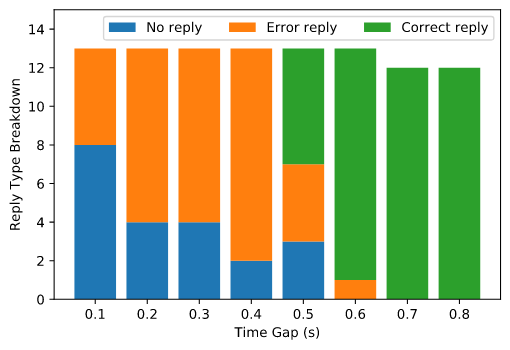
\includegraphics[scale=0.4]{../measurement/results/1207night/reply_type_breakdown}
	\caption{Bar plot showing how often Alexa replied correctly to a command for different gap lengths between the command and non-command speech.}
	\label{fig:gap}
	\vspace{-3mm}
	\end{figure}

To confirm our results, we extract the response package that Amazon server sent to Alexa and we could see a significant difference among "non-response" package, "error response" package and "correct response" package in Fig \ref{fig:postfix_variablegap_sizes}. The size of package ranged around a mean number for each specific response. The line means the size that the package ranges and the star in the middle of the line is the mean size of each type of packages. The orange one stands for "non-response" package, and the blue one stands for "error response" while the green one stands for "correct response" 

\begin{figure}[]
    \centering
    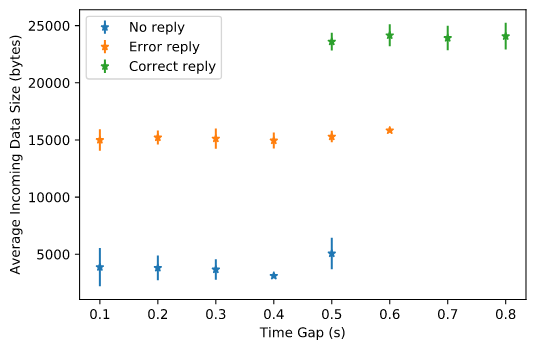
\includegraphics[width=\linewidth]{1207night/in_data_vs_gap_by_reply_type}
    \caption{Plot of the total outgoing data size against the length of the gap before non-command speech is played a command. The error bars extend to one standard deviation in either direction. Total outgoing data size is calculated as the sum of the TLS packet payload lengths going to the destination IP address with the greatest such sum.}
    \label{fig:postfix_variablegap_sizes}
\end{figure}








\subsection{"Stop" Experiment}

Following up the above experiment, in this part, we would like to detect how Alexa detects the end of a command. We would like to see whether Alexa stopped because of silence or something else.

We tried three experiment here: a) We played a background music while playing the command voice and kept playing for a while to see whether Alexa would stop transmitting package and start replying to the command. This experiment can help us figure out whether Alexa will keep recording once they detect some sounds. b) Playing the command voice with a background conversation simulates the situation in our real life. For example, in our family, when father asks something to Alexa, in the meanwhile, mother is talking something to the child. Father's voice is louder however the conversation between mother and child will keep going after father finish his command. Therefore, we would like to figure out whether Alexa can detect this situation automatically. c) We start talking immediately after the wake up world and keep talking for a while without stopping to simulate a situation that in a party there is some conversation happens around Alexa. And we want to figure out whether Alexa would stop recording automatically or will keep recording all of the sentence.

\subsection{How Alexa decided the end}

In the experiment \todo{[3]} we did an experiment to figure out how Alexa decided to stop transmitting and whether Alexa would raise privacy concern in three different kinds of situation in our life.

First, we played a background music while talking to Alexa and we found out that Alexa would stop transmitting package to Amazon server and start replying even though the music is still playing, which means Alexa can distinguish light music from human voice.

However, when we played the command voice with some conversation in the background and keep the conversation going after the command, we found out that Alexa would keep recording if there were no significant silent gap in the whole conversation, even though the conversation and command were generated by different people. As a result, Alexa is not able to detect different people's voice and stop automatically. This would suggest us not to say any private things when someone are using Alexa if we don't let them to be recorded. 

Further, when simulating the situation that few conversation happens around Alexa and someone waked up Alexa accidently, we played a full meaningless sentence with wake up word in the beginning and without any pause in it. The results turned out to be when we played a 18s sentence, the Alexa stops at 6s, 9s, 12s, 15s automatically before the sentence ends. We would assume that Alexa might stop at somewhere randomly. This result might prove that Alexa did try to protect our privacy once they figure out the voice is meaningless.

This measures the traffic streamed to server.


